\documentclass[aps,pra,twocolumn]{revtex4-1}

\usepackage{graphicx,epstopdf}
\usepackage{amsmath}
\usepackage{mathrsfs}
\usepackage{mathtools}


\begin{document}


\title{Determining the drag coefficient of the mirage rocket}

\author{Evan Anders}
\author{Andrew French}
\author{John Hoff}
\author{Michael Woodkey}
\affiliation{Department of Physics, Whitworth University, 300 W. Hawthorne Rd., Spokane, WA 99251}


\date{\today}

\begin{abstract}
Abstract goes here
\end{abstract}



\maketitle


\section{\label{section1} Introduction}
In introductory physics we learned to roughly model projectile motion using gravitational forces and initial velocities.  In advanced dynamics, we have improved upon that model by accounting for linear and quadratic drag forces.  It is our goal here to verify the correctness of drag forces by using real altitude data from a rocket launch; in verifying that this model is effective, we will determine the drag coefficient of the mirage rocket.  In section \ref{section 2}, we will examine the dynamics of a flying rocket including drag forces.  In section \ref{section 3}, we will discuss experimental setup and calibration.  In section \ref{section 4}, we will analyze the data and determine our drag coefficient.



\section{\label{section 2} Theory}
It is a good approximation to assume that drag forces act entirely in a direction opposite to that of velocity, where
\begin{equation}
\vec{f}_\text{drag} = - f(v) \hat{v}.
\end{equation}
At speeds relative to our experiment, it is a good approximation to define
\begin{equation}
f(v) = f_\text{linear} + f_\text{quadratic} = b v + c v^2 ,
\end{equation}
where $f_\text{linear}$ will arise as a result of the viscous properties of air and $f_\text{quadratic}$ is caused by the projectile pushing air particles out of its path \cite{taylor2005}.  At high speeds, such as that of our rocket, the linear term becomes insignificant.  For a long, cylindrical object whose a velocity is aligned with the area vector of the top cylinder, the value of the quadratic drag coefficient becomes
\begin{equation}
c = \gamma A = \gamma \pi r^2.
\end{equation}

The equations of motion for such a moving body subject to gravity and drag is \cite{taylor2005}
\begin{equation}
m \dot{\vec{v}} = m \vec{g} - c v \vec{v}, \label{dragC}
\end{equation}
where $g$ is the acceleration due to gravity.  Breaking the motion of our rocket into a two-dimensional plane (horizontal $x$ and vertical $y$), our equations of motion are
\begin{equation}
m \dot{v}_x  = -c v v_x \label{xafter}
\end{equation}
and
\begin{equation}
m \dot{v}_y  = -c v v_y - mg, \label{yafter}
\end{equation}
where
\begin{equation}
v = \sqrt{v_x^2 + v_y^2} \label{vValue}
\end{equation}
and $c$ is defined by Eq. (\ref{dragC}).

This system of equations is accurate for a rocket in motion \emph{after} its motor burn is completed.  Before this time, the rocket motor provides an additional force in the direction of motion, such that
\begin{equation}
\vec{f}_\text{burn} = f_\text{burn}(t) \hat{v}.
\end{equation}
During the burn, the mass of the rocket-motor system decreases.  We model mass as a function of time according to
\begin{equation}
m(t) = 
\begin{cases}
m_\text{rocket} + m_\text{fuel}\dfrac{(t_\text{burn} - t)}{t_\text{burn}}, & \text{if } t < t_\text{burn} \\ \\
m_\text{rocket} & \text{if } t \geq t_\text{burn},
\end{cases}
\end{equation}
where $m_\text{rocket}$ is the mass of the rocket plus the empty motor, $m_\text{fuel}$ is the full mass of the fuel in the motor, and $t_\text{burn}$ is the total time of the motor burn.

Acknowledging our changing masses and forces, our equations of motion become
\begin{equation}
m(t) \dot{v}_x = 
\begin{cases}
-c v v_x +  \dfrac{v_x f_\text{burn}(t)}{ v }, & \text{if } t < t_\text{burn} \\ \\
-c v v_x, & \text{if } t \geq t_\text{burn}
\label{xmotion}
\end{cases}
\end{equation}
and
\begin{equation}
m(t) \dot{v}_y = 
\begin{cases}
-c v v_y  - m(t) g+  \dfrac{v_y f_\text{burn}(t)}{ v }, & \text{if } t < t_\text{burn} \\ \\
-c v v_y - m(t) g, & \text{if } t \geq t_\text{burn},
\label{ymotion}
\end{cases}
\end{equation}
where $c$ is defined by Eq. (\ref{dragC}) and $v$ is defined by Eq. (\ref{vValue}).  Utilizing these equations, we are able to define 


\section{\label{section 3} Calibration}
\begin{figure} [t!]
	\includegraphics[width=3in]{calibration_Plot.eps}
	\caption{We hung weights from our calibration apparatus in increments of 0.5 kg and measured the force reading of our force sensor.  We conclude that our best-fit line for measured force vs. applied force is $F_\text{measured} = 0.0316F_\text{applied} + 0.00794$ N.\label{calibrationPlot}}
\end{figure}
\begin{figure} [b!]
	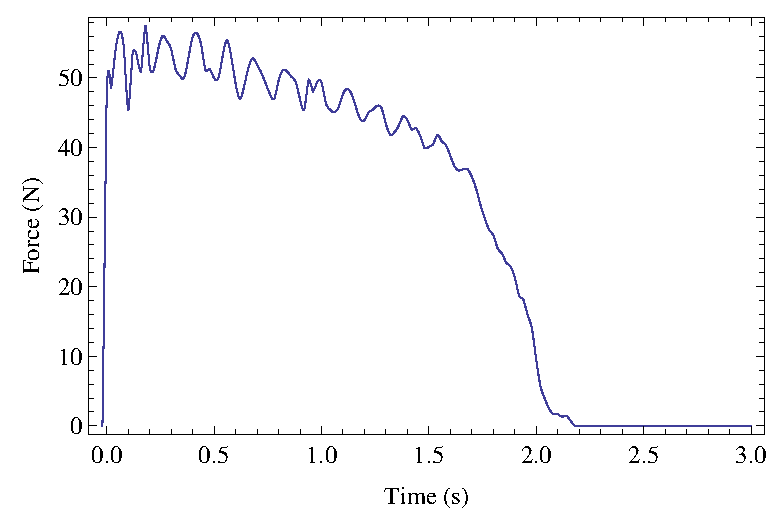
\includegraphics[width=3in]{G38-scaledTest.eps}
	\caption{The force produced by a g38 rocket motor, as measured by our calibration device and scaled by a factor of $1/0.0316$, is shown here.\label{thrustPlot}}
\end{figure}

In order to calibrate the force output of our rocket motor, we crafted a pulley-based testing apparatus and attached to a Vernier Dual-Range Force Sensor.  Due to the fact that the wire used to connect our motor to the pulley system was metal and the fact that our pulleys were neither frictionless nor massless, we determined that it was necessary to experimentally calculate the scaling factor between force applied to our calibrator and force measured by it.  We attached a mass hanger to the motor casing which hung from the pulley system, and added weight in increments of 0.5 kg, as shown in Fig. \ref{calibrationPlot}.   

We determined a relationship between measured force and applied force according to the addition of these weights, as shown by the best-fit line in Fig. \ref{calibrationPlot}.  This line follows the form
\begin{equation}
F_\text{measured} = \chi F_\text{applied} + \beta.
\end{equation}
According to our data, our force scaling factor is $\chi = 0.0316$.  We also found a small offset, $\beta = 0.00794$ N, resulting from the internal inaccuracy of our force meter, despite being zeroed.

We used the same calibration apparatus to measure the force produced by a g38 motor.  Applying a scaling factor of $F_\text{applied} \approx F_\text{measured}/(0.0316)$, we determined that the force produced by our motor peaked around $55$ N, and lasted for approximately 2.16 seconds.  The force profile of a g38 motor is shown in Fig. \ref{thrustPlot}.



\section{\label{section 4} Experimental Data and Analysis}
The mirage flew with an on-board altimeter which measured altitude as a function of pressure.  We used Wolfram Mathematica to interpolate both our flight data and our motor force data (shown in Fig. \ref{thrustPlot}).  Utilizing Eqs. (\ref{xmotion} \& \ref{ymotion}) to define the motion of our rocket, we used $\chi^2$ minimization techniques in order to determine the drag coefficient of our rocket.

Acknowledging that our flight data showed significant noise within the first second after launch, we allowed our program to vary the value of initial velocity, $v_0$ between 0 m/s and 5 m/s.  Additionally, we varied the time-step, $\Delta t$ used between the evaluation of adjacent data points between 0.05 and 0.20 seconds.  Our best fit for the drag coefficient produced a value of $\gamma =  1.21$ in Eq. (\ref{dragC}).  This value accompanied a deviation of roughly 1.3 m per point of data, where $\Delta t = 0.05$ s and $v_0 = 5$ m/s.  A comparison of our theoretical model with these values to our experimental data is shown in Fig. \ref{experiment}.

\begin{figure} [b!]
	\includegraphics[width=3in]{Mirage-G38-BestFit.eps}
	\caption{Experimental data is compared to a model of rocket flight using Eqs. (\ref{xmotion} \& \ref{ymotion}), with $v_0 = 5$ m/s, $\Delta t = 0.05$ s, and $\gamma = 1.21$.  There is a mean difference of 1.3 m between experimental and theoretical data.  \label{experiment}}
\end{figure}


\section{\label{section 5} Discussion}
We determined that the drag coefficient of our rocket was $\gamma = 1.21$.  However, this accompanied a model which allowed for an unsettling $5$ m/s of initial rocket velocity, while we know that our rocket fired from rest.  While a portion of this discrepancy may be due to the inaccuracy of the altimeter, we also failed to account for the oscillations introduced by our pulley system into our force readings.  As seen in Fig. \ref{thrustPlot}, the force delivered by the rocket is not a smooth line, but rather an oscillation of roughly 5-10 N peak-to-peak.

Additionally, we failed to measure the launch angle of our rocket.  While we ran our $\chi^2$ calculations with an estimated launch angle of $1^\circ$, we are uncertain of the accuracy of this guess, and are therefore unable to understand the $\pm 2^\circ$ that this failure to estimate the launch angle introduced to our calculations.

Final, although our model is an improvement upon the description of particle trajectories from introductory physics, we failed to account for wind resistance and other small forces (such as the friction due to the launch rail), all of which would have somewhat affected our model.

\bibliography{Bibliography}

\end{document}